\section{Graph Query Languages limitations’ on Graph Nesting}
\subsection{Graph Joins' limitations in providing the $\nu_\cong$ operator}\label{sec:whynotjoins}
\begin{figure}[!b]

\end{figure}

\begin{figure*}
	\begin{minipage}{\textwidth}
\centering
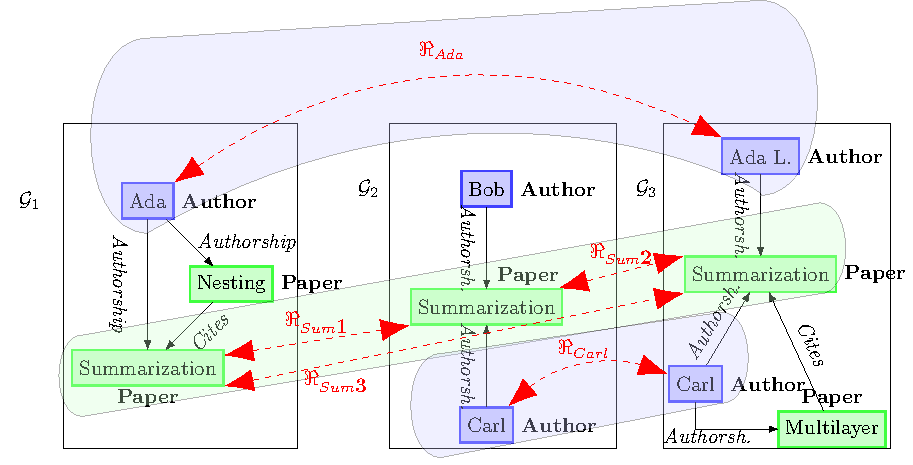
\includegraphics[width=\textwidth]{imgs/07join/discarded_leipzig/01_example}
\subcaption{Cleaned sources resulting from the
	transformation phase. The shaded areas represent distinct 
	graphs indicating which vertices (Authors and Papers) must be considered as the same entity.}
\label{fig:homog}
	\end{minipage}
	\begin{minipage}{\textwidth}

\centering
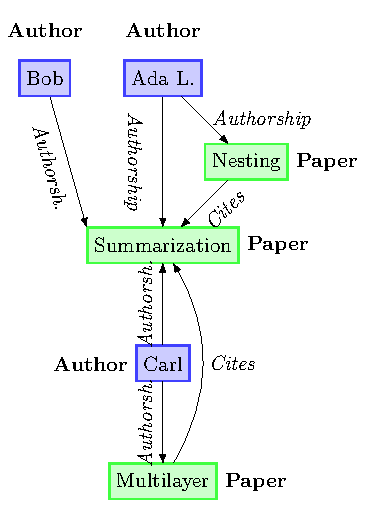
\includegraphics[scale=1]{imgs/07join/discarded_leipzig/02_result}
\subcaption{Representing the expected output $G_{out}$ for the data integration phase, ready to be fit to the graph datawarehouse.}
\label{fig:expresult}
\end{minipage}
\caption{$\nu_\cong$: another use case requiring the nesting operator $\nu$, as required by the last step of the data integration process before actually performing the queries over the integrated data. This last chapter ends the thesis by providing an example of the last operator required for such data integration process. In this case the outcome of the clustering operator is a similarity predicate $\cong$ using a entity-resolution process.}
\end{figure*}
We now discuss a use case where the graph nesting approach aggregates similar nodes into one single representation, while discarding the original sources' informations. Please refer to Section \vref{subsec:queryrw} for the general data integration scenario where such operator ($\nu_\cong$, that is grouping over an equivalence classifier $\cong$) may be adopted. In particular, we are going to show that, even though this procedure may be expressed in some cases via a full graph join, the resulting solution may be hardly implementable. In order to make our point, we are going to provide a different use case from the one previously provided.
%The following example shows that, within the graph data integration scenario, we would like to join graphs not only using functions as $\theta$ vertex predicates, but also using edges as outcomes of 

\begin{example}
	Suppose to have, within a graph ETL, three distinct bibliographic 
	sources (e.g. DBLP, Microsoft Academic Graph, Google Scholar)
	to be integrated into one final graph. 
	Each of these separately undergo a data cleaning phase
	and are represented as the distinct connected components after an entity resolution processes \cite{markus}. Such components are represented by the graphs $G_1$, $G_2$ and $G_3$ in Figure \ref{fig:homog}.
	As a next step, the entity resolution \cite{ALIEH17} analyses if there are
	nodes appearing  in the different sources and representing 
	the sam entity: as a consequence the red relations  appearing in
	Figure \ref{fig:homog} are created, and then collected into graphs representing a clique of all the resolved entities. The outcome of this operation is provided in Figure \vref{fig:expresult}, where all the entities representing one single entity are merged into one single vertex.
\end{example}

Another example where such edge joins could be of some use is within the ontology alignment process provided in Definition \vref{def:ontolalignment}: for example, we can interpret each description logic axiom $C\sqsubseteq C'$ as an oriented edge connecting each vertex of the graph satisfying the predicate $C$ to the ones satisfying $C'$, thus allowing to join two graphs which schemas were previously aligned.

	The class of  graph  $\otimes_\theta$ products could be then generalized to support edges $E$ as a basis for the definition of the $\theta$ predicates. In particular, such predicate $\theta_E$ can be defined over a set of edges $E$ as follows:
	\[\theta_E(a,b)\Leftrightarrow \exists e\in E. \lambda(e)=(a,b)\]
	In such cases we will write the predicate $\theta_E$ directly as $E$ through an abuse of notation allowing to directly list the edges involved within the join operation. We can now ask ourselves if $G_{out}$ in Figure \ref{fig:expresult} can be obtained by using the following expression:
\[(G_1\fullouterjoin^\vee_{\{\Re_{Sum1}\}}G_2)\fullouterjoin^\vee_{\{\Re_{Ada},\Re_{Sum2},\Re_{Carl}\}}G_3\]
	Let us first perform $(G_1\fullouterjoin^\vee_{\{\Re_{Sum1}\}}G_2)$ as $G_{12}$, thus merging the two \texttt{Summarization} nodes in $G_1$ and $G_2$ into a node $s_J$: we can see that we can still join the nodes linked by the edges $\Re_{Ada}$ and $\Re_{Carl}$, but we can no more join $s_J$ with the \texttt{Summarization} vertex in $G_3$, because $\Re_{Sum2}$ is not defined on $s_J$. As a consequence, we have that this way to join graphs is no more associative: if we now associate the join to the right and evaluate the following expression:
\[G_1\fullouterjoin^\vee_{\{\Re_{Sum1}\}}(G_2\fullouterjoin^\vee_{\{\Re_{Ada},\Re_{Sum2},\Re_{Carl}\}}G_3)\]
	we can now see that $\Re_{Sum1}$ is not defined over the \texttt{Summarization} node from $G_1$ and the merged node from $G_2\fullouterjoin^\vee_{\{\Re_{Ada},\Re_{Sum2},\Re_{Carl}\}}G_3$. As a consequence, these two evaluations of the edge join query provide two different results, which is disadvantageous within a computer automated environment requiring operations that can be easily scale by using associativity rules (i.e., order invariant) and that can be hence parallelized.
%	Moreover, we can furtherly generalize this concept by define the class of our graph products $\otimes_\theta$ over binary relations $\Re$: given a set of edges $E$, it is easy to define a relation $\Re_E$ as follows:
%	\[a \Re_E b \Leftrightarrow \]
	
%	operator could be extended 
%	to provide the $G_{out}$ graph in Figure \ref{fig:expresult}, by both supporting 
%	graph full joins $G\fullouterjoin_\theta G'$ and expressing the edges $R$ as
%	predicate $\theta_R$. Concerning the first extension, we have to return
%	both the mathching vertices and the non matching ones ($V\fullouterjoin_{\theta_R} V'$)
%	while, for the latter, the binary predicate $\theta_R$ should be
%	defined as $\theta_R(u,v)\Leftrightarrow (u,v)\in R$. As we will see in the following example, this trivial generalization undermines the associativity rule for graph $\theta$-joins. This problem will lead to the definition of the Graph Nesting operation in the next chapter. 
%	
%	Please note that such extended operator is not
%	associative.
%	Suppose we want to construct $G_{out}$ by composing $\fullouterjoin_{\theta_R}$ operations: 
%	when the first two graphs are joined as the intermediate result $\delta G$ (e.g. 
%	$G_1\fullouterjoin_{\theta_{\{{r}_{Sum1}\}}} G_2$), the $\theta_{R}'$ 
%	required for the final operation $\delta G_{out}\fullouterjoin_{\theta_R'}G_3=G_{out}$
%	must consider that not all the vertices in $\delta G$ are linked by ${R}$
%	(such as the nodes that have been already joined). This implies that this join operation increases
%	the number of required join comparisons, because even the ${R}$ edges have to be joined
%	in order to match the joined vertices. An
%	example of such operation is provided in Algorithm
%	\ref{alg:example}, Line \ref{alg:example:gfdj}. 
%
%
%
%As a next step we could see that we could equivalently perform the join among the vertices through
%a relation $\Re$, which expresses which vertices among the graphs are related to each other. Hereby,
%we could rewrite the previous definition as follows:
%
%\begin{definition}
%	Given two data graphs $G_1=(V_1,E_1,A_1)$ and $G_2=(V_2,E_2,A_2)$, a \textbf{general graph
%		$\Re$-join} is defined as follows:
%	\begin{gather*}
%	G_1\Join_\Re^{\textbf{es}} G_2=(V_1\Join_\Re V_2,E_{\textbf{es}},A_1\cup A_2)
%	\end{gather*}
%	where $\Re$ is a binary relation among the vertices and the $\Re$-join among the vertices
%	is defined as follows:
%	\begin{gather*}
%	V_1\Join_\Re V_2=\Set{v\oplus v''|v\in V_1, v''\in V_2, v\Re v'', (v\oplus v'')[A_1]=v, (v\oplus v'')[A_2]=v''}
%	\end{gather*}
%\end{definition}
%
%With the next example we want to show that this definition allows to both preserve
%in the graph $\Re$-join definition all the properties of the $\theta$-Join, and to
%change the result of the join operation by only changing the ``directionality'' of the relation $\Re$.

%\begin{figure}[!t]
%	\centering
%	\begin{minipage}[b]{\linewidth}
%		\centering
%		\includegraphics[scale=0.6]{imgs/07join/joinexamples/graphplanes2_mod3e}
%		\subcaption{$\Re_1$}\label{fig:reprR1}
%	\end{minipage}\\
%
%	\begin{minipage}[b]{\linewidth}
%		\centering
%		\includegraphics[scale=0.6]{imgs/07join/joinexamples/graphplanes2_mod3f}
%		\subcaption{$\Re_2$}\label{fig:reprR2}
%	\end{minipage}\\
%
%	\begin{minipage}[b]{\linewidth}
%			\centering
%			\includegraphics[scale=0.6]{imgs/07join/joinexamples/graphplanes2_mod3g}
%			\subcaption{$\Re_1'$}\label{fig:reprR1p}
%	\end{minipage}\\
%
%	\begin{minipage}[b]{\linewidth}
%		\centering
%		\includegraphics[scale=0.6]{imgs/07join/joinexamples/graphplanes2_mod}
%		\subcaption{$\Re_M$}\label{fig:reprM}
%	\end{minipage}
%
%	\caption{Representing relations as edges between $G_1$ and $G_2$}
%	\label{fig:reasedges}
%\end{figure}
%We can express any $\theta$ predicate into a relation $\Re$: Figure \ref{fig:reasedges}
%provides a graphical representation of a possible scenario.
%
%Outer joins and disjunctive $\Re$-joins could be used in ontology matching applications \cite{sndOntMatch}:
%in this use case the two graphs to be joined are the two ontologies, and $\Re$ is the result of
%the ontology matching problem, where $a\Re b$ iff. $a$'s definition is contained by $b$. By using the
%left join we could obtain as a result the left ontology enriched by the matched more general items in
%the latter ontology, while the full outer join could merge the two ontologies keeping track of the
%discrepancies (that is not allowing to merge descriptions that are only partially represented by the
%ontology). 

%The current  impossible to chain a sequence of $\Re$-join operations because $\Re$ are strictly related to the definition of the underneath data. As a consequence, $\Re$ cannot be initially definied over the to-be-joined data and, as a result, we would have to change both the relations $\Re$ and the data, thus increasing the computational costs. As we will see in the following chapter, this limitation also applies to graph grouping operations and, in order to solve this problem once and for all, we're going to provide an operator solving this problem and providing an implementation for both graph joins and graph grouping. 

Figure \ref{fig:homog} also suggests on how such an operation can be carried out: instead of performing the full outer join on the graphs stepwise, we can first perform the set union between the three graphs, and then aggregate all the elements within the same dashed area as one single vertex by using the $\nu$ nesting operator over graphs, thus motivating the requirement of such graph nesting operator.
